%!TEX root = ../main.tex

% ============================================================
%  CAPÍTULO 6: RESULTADOS
% ============================================================

\chapter{Resultados}\label{ch:resultados}

% ──────────────────────────────────────────────────────────────
\section{Resultados de Bolivia (Etapa 1)}
% ──────────────────────────────────────────────────────────────

La replicación del enfoque de \textit{nowcasting} electoral basado en encuestas sobre la segunda vuelta presidencial boliviana (Paz vs. Quiroga, octubre de 2025) arrojó resultados mixtos que confirmaron las limitaciones estructurales de este paradigma y justificaron el viraje metodológico hacia la Etapa~2.

\subsection*{Datos y configuración experimental}

Se construyó un \textit{dataset} de 308 observaciones diarias (26 columnas de características) que combinaba métricas diarias de interacción, \textit{posts}, \textit{likes}, \textit{shares} y comentarios, de Facebook, Instagram, TikTok y Twitter/X para ambos candidatos. La variable objetivo fue la intención de voto real interpolada a partir de las encuestas publicadas entre la primera y la última medición demoscópica disponible. El resultado real del 19 de octubre de 2025 fue: \textbf{Paz: 54{,}53\%}, \textbf{Quiroga: 45{,}47\%}.

\subsection*{Comparativa de modelos}

Se evaluaron seis modelos (más el \textit{baseline} de última encuesta) sobre su predicción en el día de elecciones. La Tabla~\ref{tab:bolivia_metricas} resume las métricas para el candidato Paz (el ganador), que son las más relevantes para la predicción. La Figura~\ref{fig:bolivia_mlp_pca} ilustra la evolución temporal del mejor modelo.

\begin{table}[htbp]
\centering
\caption{Métricas de predicción en el día de elecciones: candidato Paz (real: 54{,}53\%)$^\dagger$}
\label{tab:bolivia_metricas}
\begin{tabular}{l c c c}
\toprule
\textbf{Modelo} & \textbf{Predicción Paz} & \textbf{MAE} & \textbf{MAPE} \\
\midrule
Baseline (última encuesta)    & 36{,}50\% & 0{,}1803 & 33{,}1\% \\
Regresión Lineal              & 24{,}85\% & 0{,}2968 & 54{,}4\% \\
Regresión Lineal + PCA        & 23{,}38\% & 0{,}3115 & 57{,}1\% \\
MLP-BP                        & 46{,}91\% & 0{,}0762 & 14{,}0\% \\
\textbf{MLP-BP + PCA}         & \textbf{51{,}74\%} & \textbf{0{,}0279} & \textbf{5{,}1\%} \\
GRNN                          & 34{,}67\% & 0{,}1986 & 36{,}4\% \\
GRNN + PCA                    & 34{,}48\% & 0{,}2005 & 36{,}8\% \\
\bottomrule
\end{tabular}
\vspace{0.5em}
\begin{minipage}{0.92\textwidth}
\footnotesize $^\dagger$ Las métricas se calcularon sobre el único punto observable fuera de muestra: la predicción del día de la elección vs.~el resultado certificado. Por construcción matemática, MAE = RMSE cuando $n=1$; la columna RMSE se omite por ser redundante. A modo de referencia heurística, el error de predicción en el día de la elección (2{,}79 pp) es aproximadamente 1{,}2 veces el error medio del modelo sobre las 14 fechas de encuesta disponibles ($\approx 6{,}2$ pp). Este cociente sugiere que la predicción puntual no fue atípicamente precisa respecto a la calibración general del modelo; sin embargo, dado que el conjunto de prueba consta de un único punto, esta comparación tiene carácter ilustrativo y no constituye una medida formal de generalización.
\end{minipage}
\end{table}

El modelo \textbf{MLP-BP + PCA} fue el único que superó al \textit{baseline}: predijo un 51{,}74\% para Paz (error absoluto de solo 2{,}79 puntos porcentuales frente al resultado real de 54{,}53\%), mejorando más de seis veces al estimador inercial de última encuesta (MAE = 0{,}1803). Los modelos de regresión lineal fallaron de manera categórica, incluso invirtiendo el resultado (prediciendo a Quiroga como ganador con 75{,}15\%), lo que confirma que la relación entre interacciones digitales e intención de voto no es lineal. El GRNN quedó sistemáticamente ``atascado'' sobreestimando a Quiroga durante toda la serie temporal (véase Figura~\ref{fig:bolivia_mlp_pca}).

\begin{figure}[htbp]
    \centering
    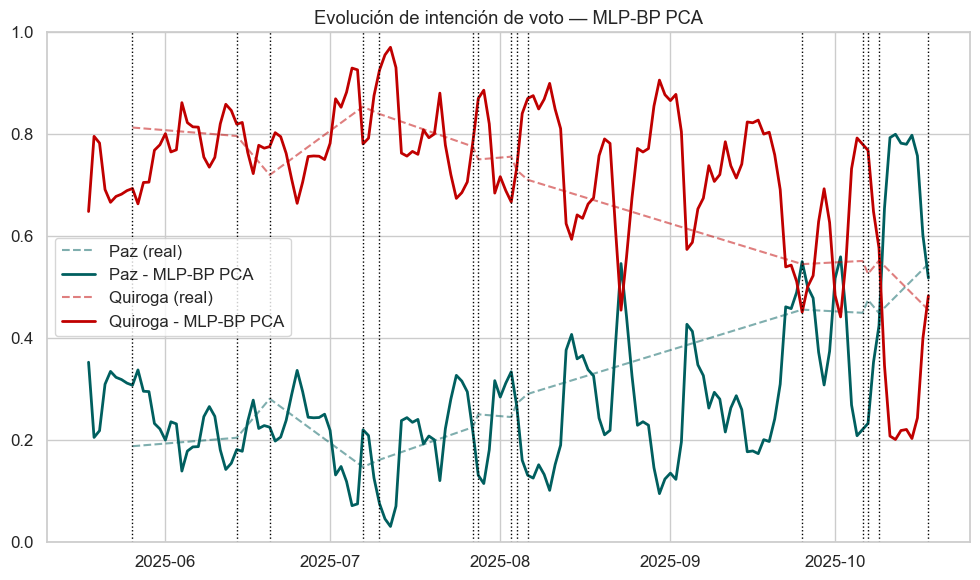
\includegraphics[width=\textwidth]{img/bolivia_model_MLP-BP_PCA.png}
    \caption{Evolución diaria de la intención de voto estimada por el modelo MLP-BP+PCA (líneas continuas) vs. la intención de voto real interpolada desde encuestas (líneas discontinuas) para Paz (verde) y Quiroga (rojo). Las líneas verticales punteadas marcan la fecha de publicación de cada encuesta. El modelo captura la tendencia ascendente de Paz en las últimas semanas, aunque con alta varianza diaria.}
    \label{fig:bolivia_mlp_pca}
\end{figure}

\subsection*{Limitaciones estructurales identificadas}

A pesar del resultado numérico del MLP-BP+PCA, el análisis reveló tres falencias críticas que desaconsejaron continuar esta ruta:

\begin{enumerate}
    \item \textbf{Falta de generalización}: Los pesos y la topología de la red neuronal son específicos de este evento electoral. No existe mecanismo para transferir el aprendizaje a otra contienda sin reentrenamiento completo, haciendo el modelo irrepetible.

    \item \textbf{Ceguera ante giros súbitos}: Los cambios de favorabilidad ocurridos en la última semana de campaña, cuando Paz remontó significativamente en las encuestas, no fueron capturados por las métricas de interacciones acumuladas. El modelo operó con un rezago estructural irrecuperable.

    \item \textbf{Disociación de la señal TikTok}: Un análisis de importancia de variables identificó que la dinámica de viralidad de TikTok operaba en un plano desacoplado del resto de plataformas. Los picos de interacción en TikTok inyectaban varianza espuria en momentos en que la intención de voto real permanecía estacionaria, degradando la señal agregada.
\end{enumerate}

Un experimento adicional con \textit{lag features} (memorias de 1, 2 y 3 días) y ponderación temporal exponencial (mayor peso a días recientes) buscó dotar al modelo de capacidad para detectar cambios de tendencia. Si bien este enfoque redujo el sesgo en períodos de alta actividad, amplificó el ruido diario y no logró resolver la inestabilidad en los días de elección. Estos hallazgos consolidaron la decisión de redirigir el enfoque hacia un modelo de regresión fraccional elección-agnóstico, independiente de las dinámicas específicas de un único evento.



% ──────────────────────────────────────────────────────────────
\section{Resultados de Costa Rica (Etapa 2)}
% ──────────────────────────────────────────────────────────────

El modelado paramétrico del crecimiento de interacciones resolvió satisfactoriamente el obstáculo estructural que impide explotar registros históricos sin infraestructura activa de extracción. El panel de 30 días (15 antes y 15 después del día de elecciones), recogido con cadencia diaria sobre las cuatro plataformas hegemónicas, produjo \textbf{1.922 publicaciones válidas} y \textbf{19.439 observaciones} con las que se calibraron los parámetros del modelo Weibull.

\subsection*{Morfología del crecimiento: ganadores y no ganadores}

Un hallazgo central del análisis es que la \textbf{curva de crecimiento acumulado de interacciones es morfológicamente idéntica entre la candidata ganadora y el resto de los competidores} (véase Figura~\ref{fig:ganadora_vs_resto} en la sección de metodología). En ambos grupos, más del 80\% de las interacciones totales se acumulan en los primeros 2--3 días desde la publicación, y a partir del Día~7 la curva es prácticamente plana. Las pruebas T día a día confirman que el crecimiento es estadísticamente significativo ($p < 0{,}0001$) hasta el Día~10, pero empíricamente irrelevante ($< 2\%$ diario) a partir del Día~5--7.

Este resultado tiene una implicación metodológica crítica: \textbf{el patrón de crecimiento orgánico es una propiedad de la plataforma, no del candidato ni del resultado electoral}. Esto valida el supuesto de estacionariedad del modelo Weibull y permite aplicar los mismos parámetros calibrados en Costa Rica 2026 para reconstruir históricamente las interacciones de cualquier otra elección.

\subsection*{Precisión proyectiva del modelo Weibull}

Los parámetros calibrados ($k$, $\alpha$, $t_0$) para cada plataforma se detallan en la Tabla~\ref{tab:weibull_params}. La evaluación de precisión se realizó simulando el escenario real de uso: tomando la medición de un día $t$ y estimando el total final como $\hat{N} = n_t / F(t; k, \alpha, t_0)$. Los resultados del MAPE mediano se resumen en la Tabla~\ref{tab:mape_plataforma} y se visualizan en la Figura~\ref{fig:error_estimacion}.

Los resultados son robustos en la mayoría de las plataformas. Al observar una publicación en su \textbf{Día~3}:

\begin{itemize}
    \item \textbf{Facebook}: MAPE mediano de \textbf{2{,}12\%} -- prácticamente sin error desde el día 3.
    \item \textbf{TikTok}: MAPE mediano de \textbf{5{,}94\%} -- muy por debajo del umbral de referencia del 20\%.
    \item \textbf{Twitter/X}: MAPE mediano de \textbf{0{,}38\%} -- error casi nulo; las publicaciones de Twitter se saturan en horas.
    \item \textbf{Instagram}: MAPE mediano de \textbf{12{,}06\%} -- el más alto, explicado por la extrema concentración de interacciones en las primeras horas (offset $t_0 = 0{,}04$ días = 1 hora).
\end{itemize}

En términos globales, entre el 89\% y el 99\% de las publicaciones (según la plataforma) se estiman con un error inferior al 20\% al observarlas en el Día~3. A partir del \textbf{Día~7}, el error mediano cae por debajo del 4\% en todas las plataformas.

\begin{table}[htbp]
\centering
\caption{MAPE mediano (\%) en la estimación del total final de interacciones, por plataforma y día de observación (panel longitudinal Costa Rica 2026).}
\label{tab:mape_plataforma}
\begin{tabular}{l c c c c c}
\toprule
\textbf{Plataforma} & \textbf{Día 0} & \textbf{Día 1} & \textbf{Día 2} & \textbf{Día 3} & \textbf{Día 7} \\
\midrule
Facebook   & 11{,}27\% &  6{,}92\% & 3{,}73\% & 2{,}12\% & 0{,}32\% \\
Instagram  & 64{,}77\% & 20{,}72\% &15{,}67\% &12{,}06\% & 3{,}76\% \\
TikTok     & 25{,}36\% & 14{,}20\% & 8{,}35\% & 5{,}94\% & 2{,}29\% \\
Twitter/X  & 56{,}37\% & 11{,}09\% & 2{,}55\% & 0{,}38\% & 0{,}00\% \\
\bottomrule
\end{tabular}
\end{table}


\subsection*{Función de reconstrucción histórica}

Con los parámetros calibrados se implementó y validó la \textbf{función de reconstrucción histórica} (véase Figura~\ref{fig:ejemplos_reconstruccion}), que dado el total de interacciones observado en un día $t$ y la plataforma, genera la curva diaria completa de interacciones nuevas e infiere el estado del post en cualquier fecha pasada. No se documentaron violaciones de monotonicidad (una publicación nunca pierde interacciones al retroceder en el tiempo), y el error mediano inyectado a la serie temporal en el Día~14 pre-elección es matemáticamente cero para Facebook y Twitter/X.



% ──────────────────────────────────────────────────────────────
\section{Resultados de Colombia (Etapa 3)}
% ──────────────────────────────────────────────────────────────

\subsection{Señal digital y correlación con el voto}

La evaluación del ecosistema digital de las elecciones de alcaldes de 2023 sobre las 31 ciudades competitivas colombianas confirmó la hipótesis fundacional del estudio: las interacciones en redes sociales albergan una señal predictiva real y cuantificable sobre el comportamiento en urnas.

Los candidatos ganadores evidenciaron una mayor mediana de \textit{engagement} por publicación que sus contendientes derrotados ($p = 0{,}0481$, prueba U de Mann-Whitney sobre la muestra mancomunada). Para controlar la dependencia intra-contienda derivada del anidamiento de los 120 candidatos en las 31 ciudades, se evaluó una prueba de permutación dentro de contienda intercambiando las etiquetas de ganador/perdedor dentro de cada municipio en 10.000 iteraciones (semilla = 42). El estadístico observado fue una diferencia de medianas de 112 puntos de \textit{engagement}; ninguna de las 10.000 permutaciones igualó o superó ese valor, arrojando un p-valor empírico $p < 0{,}0001$, lo que ratificó la significancia de la ventaja digital con mayor contundencia que el test mancomunado. Asimismo, la \textbf{dominancia relativa} de \textit{likes} ($\rho = 0{,}70$ mancomunado sobre todos los candidatos, véase la Figura~\ref{fig:col_scatter}) superó ampliamente al volumen nominal de interacciones ($\rho \approx 0{,}45$) como predictor de la cuota electoral. Un heurístico ingenuo basado en asignar la victoria al candidato con mayor dominancia de \textit{engagement} acertó en el 71{,}0\% de las 31 contiendas (22 de 31 aciertos, IC 95\% de Wilson: 53{,}4\%--83{,}9\%). Dado que dominancia y cuota son variables composicionales que comparten denominador dentro de cada contienda, se cuantificó la inflación mecánica del coeficiente de Spearman mediante una segunda prueba de permutación: en 10.000 iteraciones se redistribuyeron aleatoriamente los \textit{likes} entre candidatos dentro de cada municipio, preservando el total de \textit{likes} por ciudad pero eliminando la relación entre \textit{likes} y votos. El $\rho$ promedio bajo esa hipótesis nula composicional fue $\rho_{\text{mec.}} = 0{,}261$ (IC empírico al 95\%: hasta $0{,}397$), lo que implica que aproximadamente el 39\% del $\rho$ observado se debe a la mecánica composicional y el 61\% restante ($\rho_{\text{real}} \approx 0{,}41$) constituye señal predictiva genuina entre \textit{likes} y votos. Ninguna de las 10.000 permutaciones de \textit{likes} alcanzó el $\rho$ observado ($p < 0{,}0001$). Esta descomposición confirma que la advertencia composicional reduce la magnitud del $\rho$ pero no invalida la relación; la validez predictiva fuera de muestra la establece el protocolo LOCO-CV.

\begin{figure}[htbp]
\centering
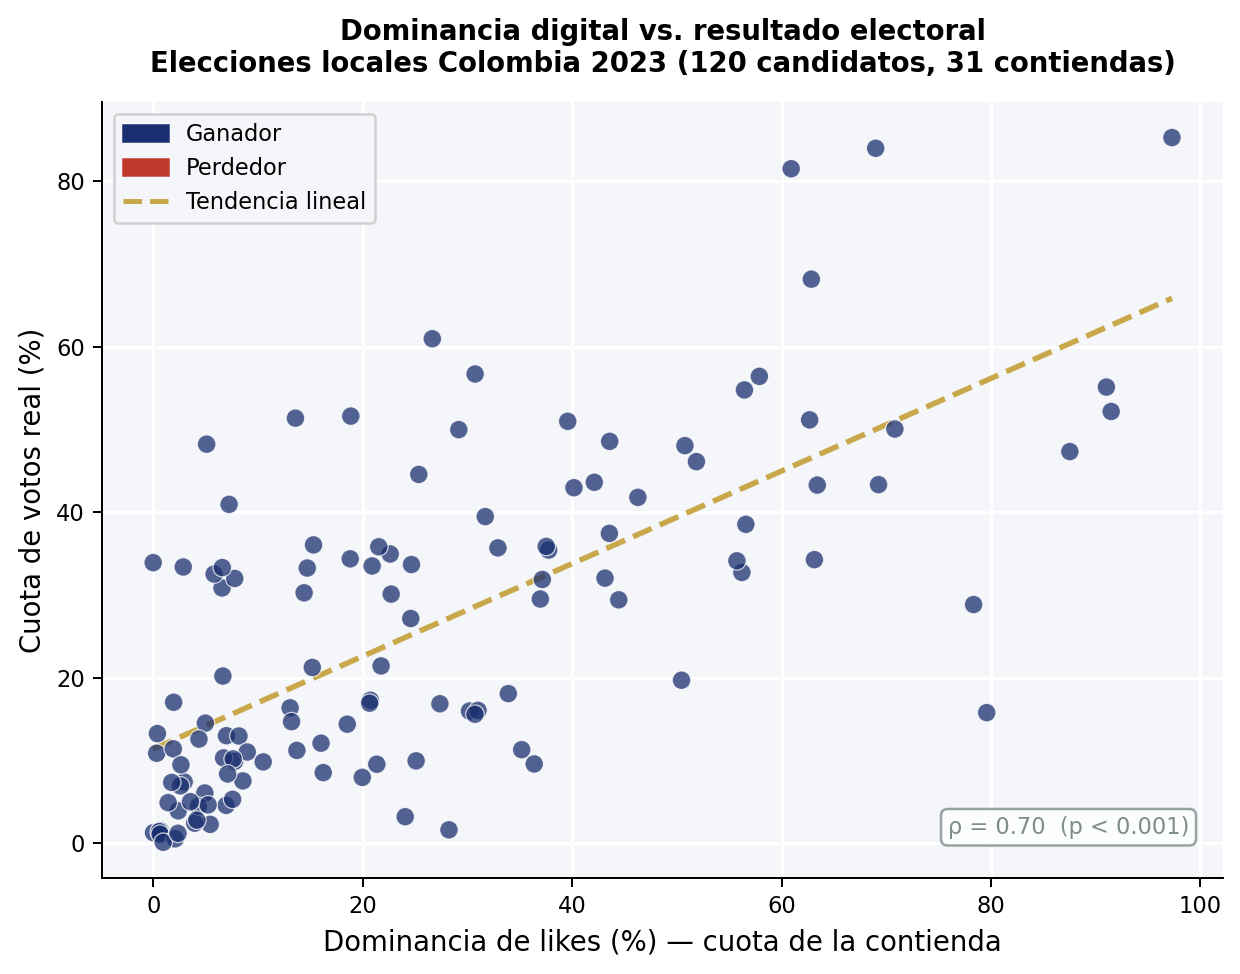
\includegraphics[width=0.82\linewidth]{img/col_scatter_dominancia_votos.png}
\caption{Relación entre la dominancia digital de \textit{likes} y la cuota de voto real en las elecciones de alcaldes de Colombia 2023 (120 candidatos, 31 contiendas). La correlación de rango de Spearman calculada sobre todos los candidatos (mancomunada) es $\rho = 0{,}70$ ($p < 0{,}001$). Los puntos azules corresponden a ganadores y los rojos a perdedores.}
\label{fig:col_scatter}
\end{figure}

\subsection{Modelo de regresión fraccional}

El modelo de regresión logística fraccional entrenado sobre los 120 candidatos (31 contiendas) produjo, mediante validación \textit{leave-one-contest-out} (LOCO-CV), los resultados que se resumen junto al resto de especificaciones evaluadas en la Tabla~\ref{tab:automl_escalera}.

\begin{table}[htbp]
\centering
\caption{Escalera de resultados del proceso AutoML acotado: comparativa completa de especificaciones (LOCO-CV, 31 contiendas, 120 candidatos).}
\label{tab:automl_escalera}
\begin{tabular}{l c c c}
\toprule
\textbf{Modelo} & \textbf{MAE (pp)} & \textbf{$R^2_{oos}$} & \textbf{Top-1} \\
\midrule
\textit{Baseline} proporcionalidad & 12{,}61 & 0{,}185 & 71{,}0\% \\
Núcleo digital (solo logit\_likes) & 11{,}52 & 0{,}460 & 71{,}0\% \\
\textbf{Modelo completo (ElasticNet, selección anidada)} & \textbf{9{,}56} & \textbf{0{,}518} & 64{,}5\% \\
\textit{Gradient boosting} superficial (control) & 9{,}91 & 0{,}515 & 67{,}7\% \\
\bottomrule
\end{tabular}
\end{table}

El modelo completo con selección anidada ElasticNet reduce el MAE en 3{,}05~pp respecto al \textit{baseline} de proporcionalidad y en 1{,}96~pp respecto al núcleo digital, alcanzando un MAE de \textbf{9{,}56~pp} y un $R^2_{oos}$ de 0{,}518. La Figura~\ref{fig:col_mae} ilustra la escalera de mejora entre especificaciones. El \textit{gradient boosting} de control (MAE~9{,}91) no logra superar a la regresión regularizada, confirmando que con 31 contiendas la no-linealidad adicional solo añade varianza. El descenso del \textit{top-1} al 64{,}5\% es teóricamente coherente: optimizar para la cuota de voto de \textit{todos} los candidatos y acertar quién es el \#1 son objetivos distintos, y el modelo sacrifica algo de exactitud de ranking a cambio de estimaciones de magnitud más calibradas.

\begin{figure}[htbp]
\centering
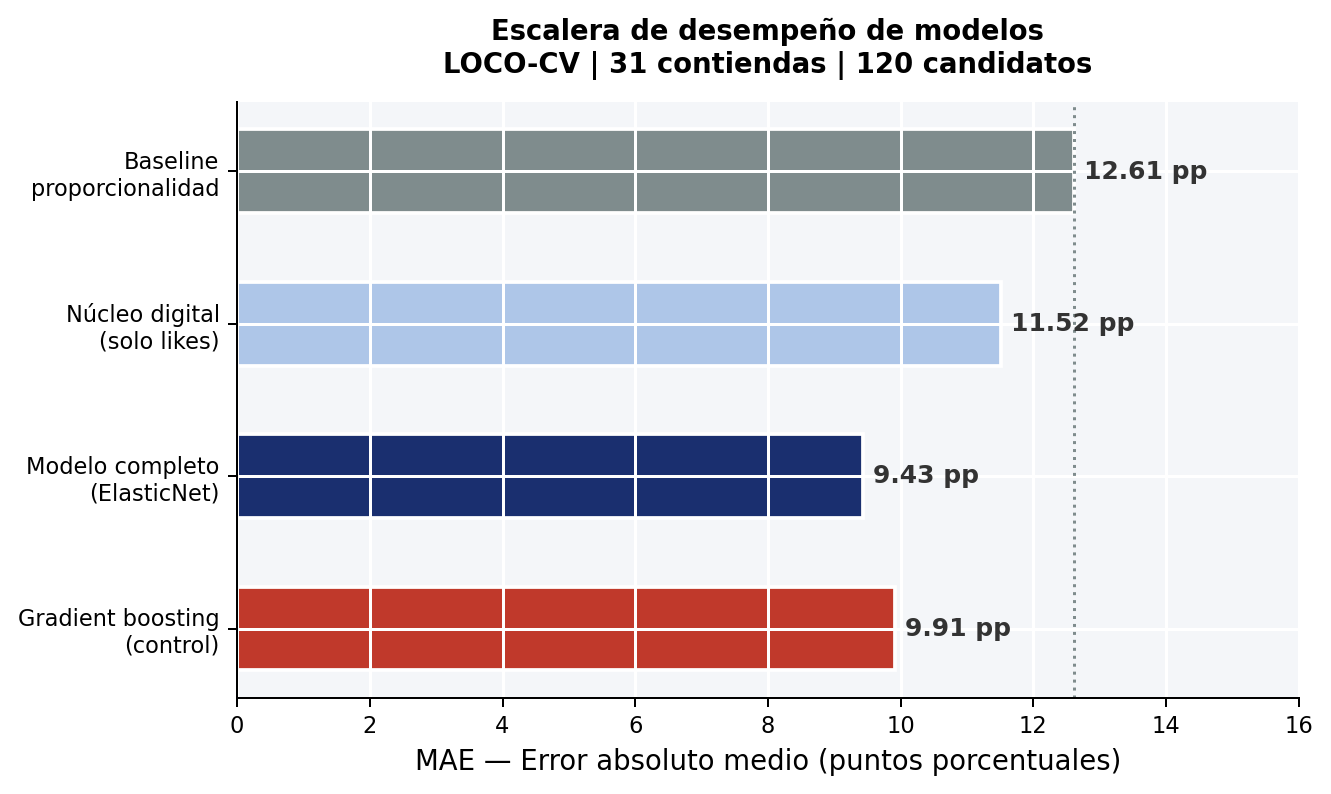
\includegraphics[width=0.82\linewidth]{img/col_mae_escalera.png}
\caption{Escalera de desempeño de especificaciones evaluadas (LOCO-CV, 31 contiendas). Cada barra representa el MAE en puntos porcentuales de la cuota de voto. La línea punteada vertical marca el \textit{baseline} de proporcionalidad.}
\label{fig:col_mae}
\end{figure}

\subsection{Especificación ganadora ElasticNet}

La selección anidada de especificación por LOCO-CV identificó como modelo óptimo el ElasticNet regularizado con dos predictores: la dominancia en logit de \textit{likes} ($f_{\text{likes\_dom}}$) y su interacción con el logaritmo de la población municipal ($f_{\text{likes\_dom}} \times (\log\text{pob} - \overline{\log\text{pob}})$). Los coeficientes estimados fueron $\hat{\beta}_1 = 0{,}111$ y $\hat{\beta}_2 = 0{,}026$, con intercepto $0{,}258$ e hiperparámetros \textit{alpha} $= 0{,}0475$ y \textit{L1 ratio} $= 0{,}10$.

La interpretación del moderador de población es teóricamente coherente: en municipios grandes, dominar las redes se traduce con más fuerza en votos que en municipios pequeños, porque la población no actúa como efecto directo (es constante dentro de la contienda y se diluye) sino como \textbf{moderador} de cuánto pesan las interacciones. En la especificación ganadora de dos predictores, los coeficientes en escala estandarizada son $\hat{\beta}_1 = 0{,}111$ (dominancia) y $\hat{\beta}_2 = 0{,}026$ (moderador), retenidos en el 100\% de los pliegues. La Figura~\ref{fig:col_coef} ilustra la magnitud y la estabilidad inter-pliegue de los coeficientes en la especificación final.

\begin{figure}[htbp]
\centering
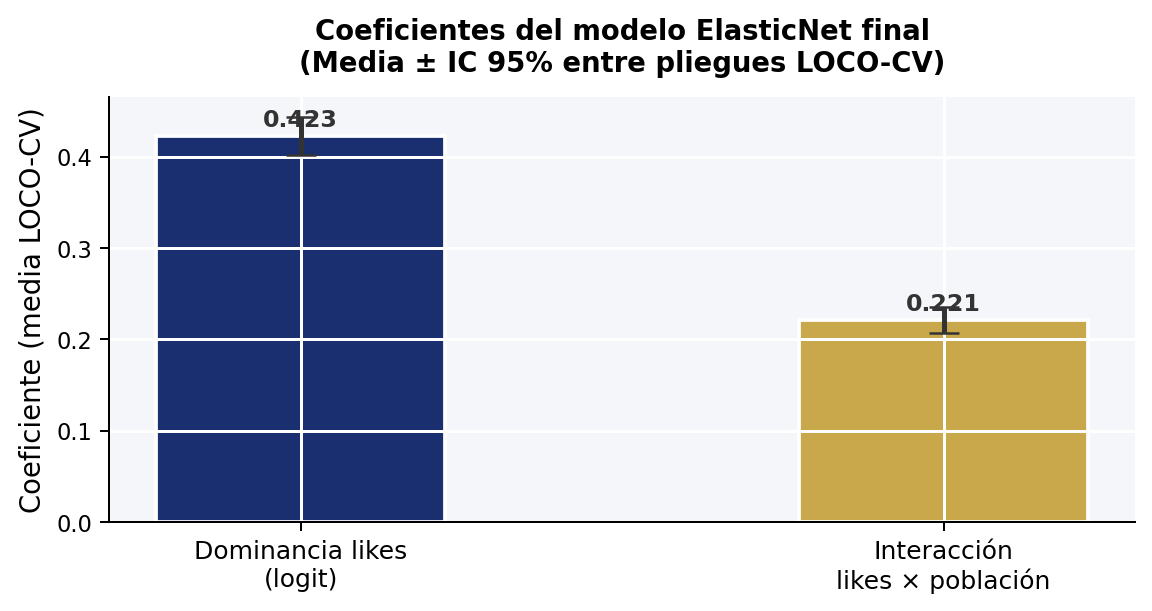
\includegraphics[width=0.72\linewidth]{img/col_coef_bootstrap.png}
\caption{Estabilidad de los coeficientes del modelo de dos variables (GLM fraccional, \textit{link} logit) estimados entre los 31 pliegues LOCO-CV en escala logit ($\hat{\beta}_1 \approx 0{,}780$ para la dominancia de \textit{likes} y $\hat{\beta}_2 \approx 0{,}540$ para el moderador de población, barras con media $\pm$ IC 95\%). En escala estandarizada con \textit{StandardScaler}, corresponden a $\hat{\beta}_1 = 0{,}111$ y $\hat{\beta}_2 = 0{,}026$ en la especificación final (Sección~5.6.b).}
\label{fig:col_coef}
\end{figure}

La Figura~\ref{fig:col_residuals} compara las predicciones del modelo con los resultados reales y muestra la distribución de residuos, confirmando que el error es aproximadamente simétrico y centrado en cero.

\begin{figure}[htbp]
\centering
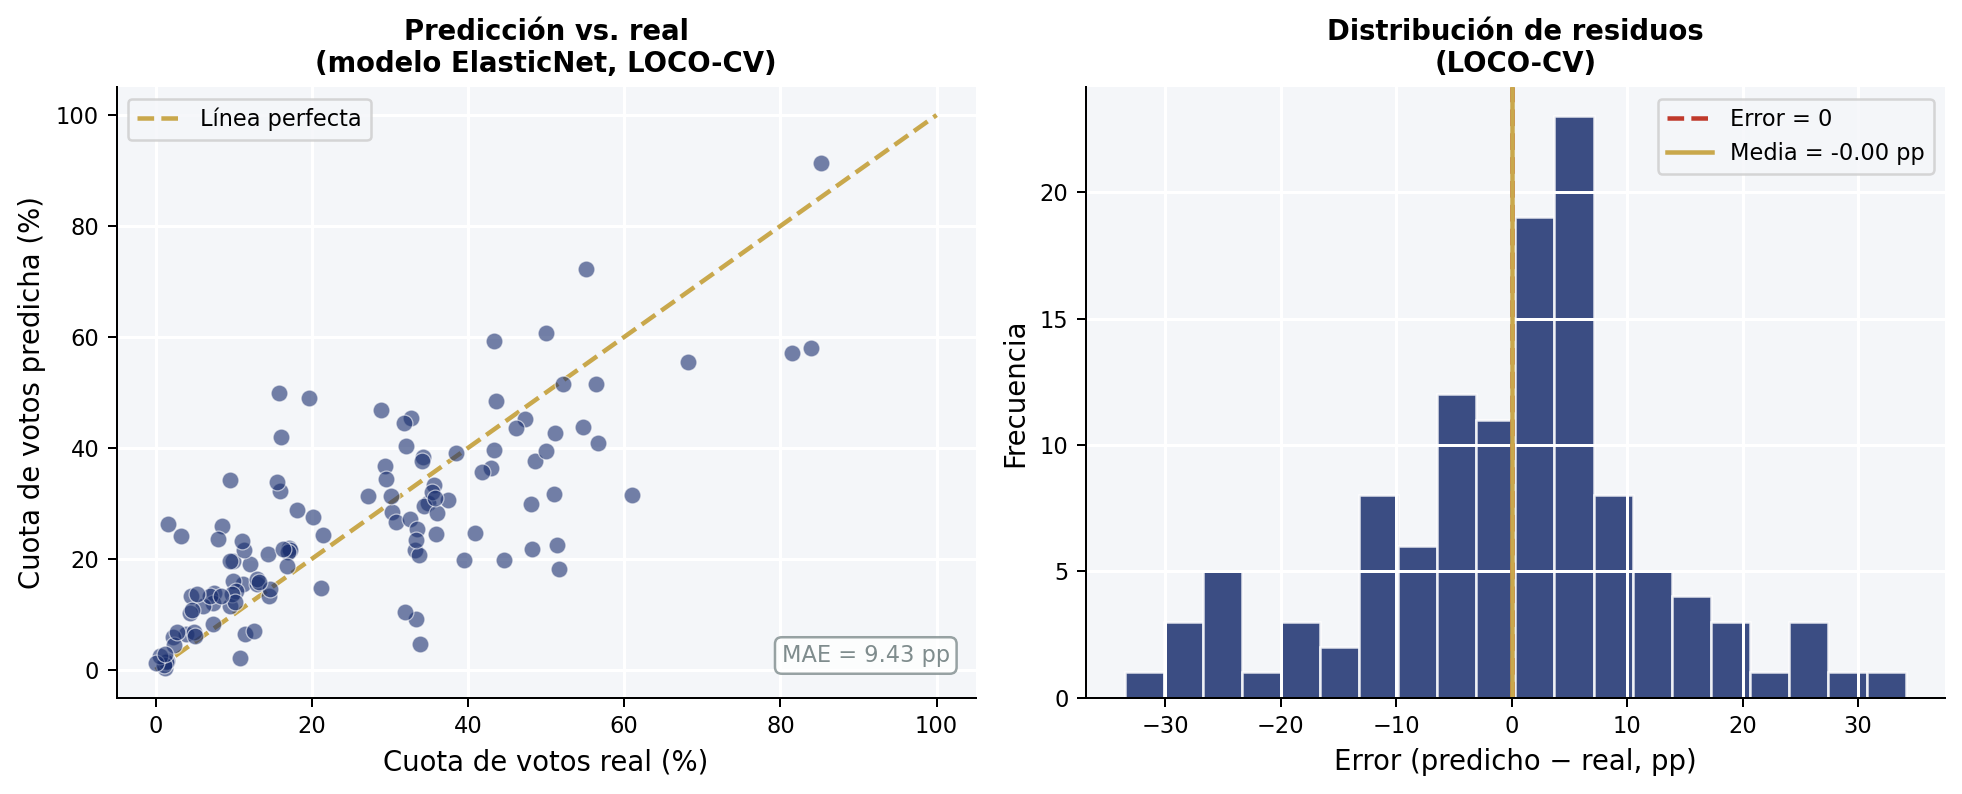
\includegraphics[width=0.95\linewidth]{img/col_loco_residuals.png}
\caption{Izquierda: predicción vs. resultado real para los 120 candidatos en validación LOCO-CV. La línea discontinua dorada representa la predicción perfecta. Derecha: distribución de residuos (predicho $-$ real, en pp); la línea roja marca el error cero y la dorada la media del error.}
\label{fig:col_residuals}
\end{figure}

El modelo final tiene en la práctica \textbf{dos versiones complementarias}: (i) la \textbf{especificación de dos predictores} ($f_{\text{likes\_dom}}$ más el moderador de interacción con la población), que es la que se entrenó sobre las 31 contiendas y se validó prospectivamente en la presidencial 2026, con MAE fuera de muestra de \textbf{9{,}56~pp} (LOCO-CV); y (ii) el \textbf{ElasticNet sobre el \textit{pool} completo} de nueve variables, que con selección anidada alcanza un MAE de 9{,}57~pp pero retiene variables territoriales específicas del nivel municipal (población, número de candidatos) que no son directamente transferibles a una elección nacional de dos candidatos.

\subsection{Aplicación a la Segunda Vuelta Presidencial 2026}

El 21 de junio de 2026 se celebró la segunda vuelta presidencial de Colombia, enfrentando a Iván Cepeda Castro y Abelardo De la Espriella. El modelo ELA-NOM, sin reentrenamiento, produjo el pronóstico que resume la Tabla~\ref{tab:pronostico_2026}.

\begin{table}[htbp]
\centering
\caption{Pronóstico ELA-NOM vs.~resultado real de la segunda vuelta presidencial colombiana (21 jun.~2026). Fuente del resultado: Registraduría Nacional del Estado Civil.}
\label{tab:pronostico_2026}
\begin{tabular}{l c c c c}
\toprule
\textbf{Candidato} & \textbf{\textit{Likes} totales} & \textbf{Dom.~\textit{likes}} & \textbf{Pronóstico} & \textbf{Resultado real} \\
\midrule
Iván Cepeda Castro & 17.087.679 & 77{,}6\% & 60{,}5\% & 49{,}52\% \\
Abelardo De la Espriella & 4.926.361 & 22{,}4\% & 39{,}5\% & 50{,}48\% \\
\bottomrule
\end{tabular}
\end{table}

\begin{figure}[htbp]
\centering
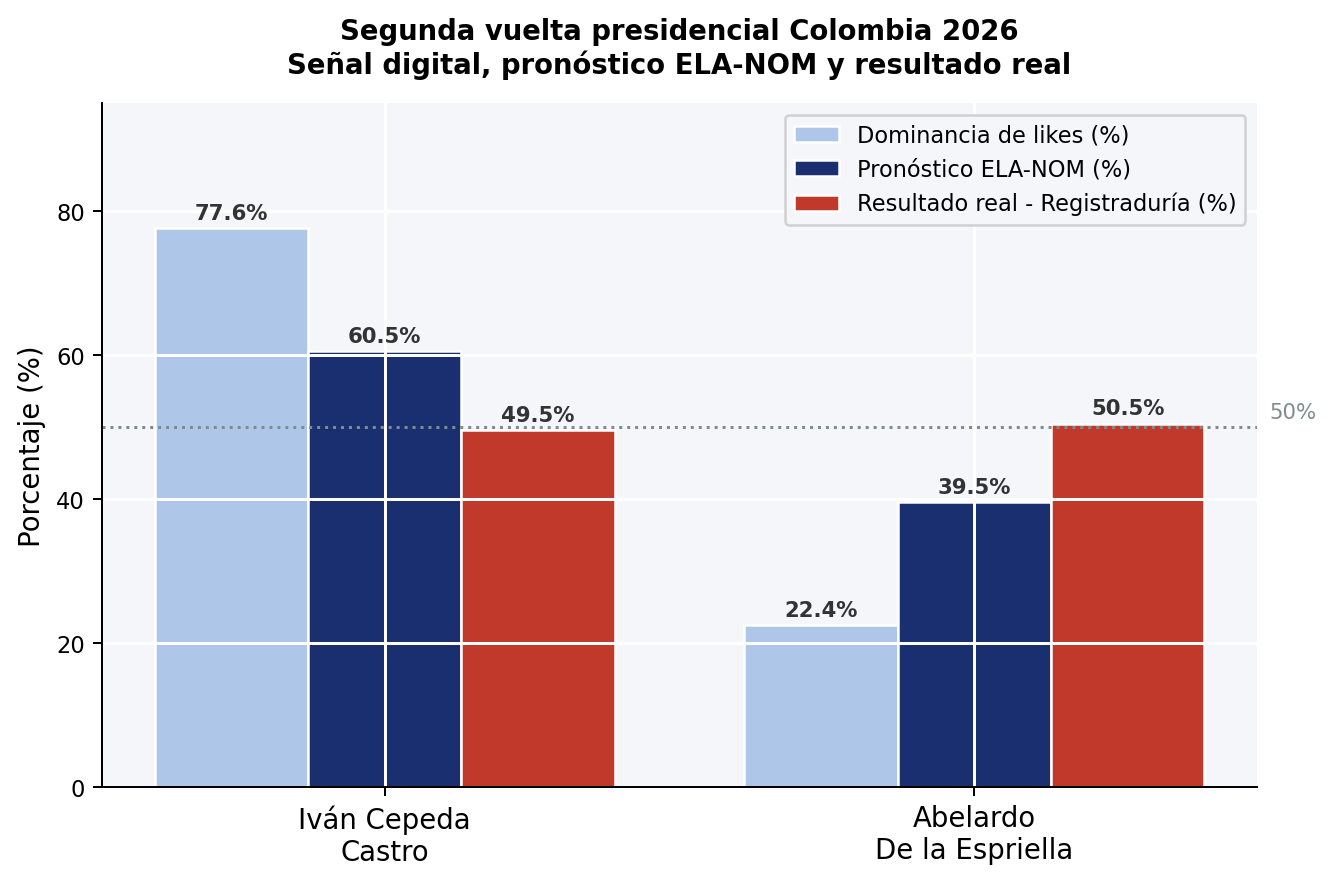
\includegraphics[width=0.82\linewidth]{img/col_dominancia_2026.png}
\caption{Comparación entre la señal digital (dominancia de \textit{likes}), el pronóstico de ELA-NOM y el resultado certificado por la Registraduría Nacional del Estado Civil en la segunda vuelta presidencial de Colombia (21 jun.~2026).}
\label{fig:col_2026}
\end{figure}

El modelo apuntó correctamente la dirección de la señal digital (Cepeda acumuló 3{,}5 veces más \textit{likes}), pero sobreestimó la ventaja resultante. El pronóstico del 60{,}5\% se obtuvo aplicando la fórmula de re-centrado para segunda vuelta: se calculó la señal estandarizada ($\hat{s} = \hat{\beta}_1 \cdot z_{\text{dom}} + \hat{\beta}_2 \cdot z_{\text{mod}} = 0{,}2294$), se sumó a la base de 50\% ($0{,}50 + 0{,}2294 = 0{,}729$) y se normalizó entre los dos candidatos ($0{,}729 / (0{,}729 + 0{,}477) = 60{,}5\%$). El error absoluto fue de \textbf{10{,}98~pp} (60{,}5\% pronóstico vs.~49{,}52\% real), superando el MAE medio fuera de muestra del modelo de dos predictores aplicado (9{,}56~pp sobre las 31 contiendas municipales de entrenamiento).

El dato definitivo para contextualizar el error es el margen real de la elección: De la Espriella ganó por \textbf{apenas 0{,}96 puntos porcentuales} (50{,}48\% vs.~49{,}52\%), es decir, una contienda de empate técnico. Predecir correctamente el ganador en semejante escenario excede la resolución de cualquier modelo basado en métricas de \textit{engagement} agregado y, de hecho, excede la resolución de la mayoría de las encuestas publicadas durante la campaña. El error observado (10{,}98~pp) supera en \textbf{1{,}42~pp} el MAE medio del modelo (9{,}56~pp): este caso queda por fuera del límite de resolución empírico del modelo, lo que confirma que la contienda se encontraba en un territorio donde ningún sistema basado en \textit{engagement} agregado tiene precisión suficiente para determinar el ganador.

Este hallazgo delimita con precisión el espacio donde ELA-NOM es informativo: contiendas con ventajas digitales netas superiores a 20~pp, donde la señal digital traslada más fuerza a las urnas. En contiendas de empate técnico como la segunda vuelta de 2026, las métricas de \textit{engagement} agregado capturan movilización simbólica pero no la movilización efectiva diferencial, los giros de última semana ni la estructura organizativa territorial. Lejos de invalidar el modelo, este resultado es el límite estructural mejor documentado que la investigación puede reportar.

\subsection{Análisis complementario: tamaño de muestra y tracción tardía}

Las dos preguntas derivadas evaluadas computacionalmente arrojan conclusiones que merecen una lectura honesta y calibrada.

\subsubsection*{P4: \textquestiondown{}Cuántas contiendas de entrenamiento son necesarias para estabilizar el rendimiento del modelo?}

Para responder esta pregunta se realizó un experimento de curva de aprendizaje: se repitió 50~veces la estimación del MAE fuera de muestra variando el número de contiendas de entrenamiento entre 5 y 30 (con semilla aleatoria fija \texttt{seed=42}). Los resultados se muestran en la Tabla~\ref{tab:learning_curve} y en la Figura~\ref{fig:col_learning_curve}.

\begin{table}[htbp]
\centering
\caption{Curva de aprendizaje: MAE fuera de muestra según el número de contiendas de entrenamiento (50 repeticiones con muestreo aleatorio, semilla 42). Modelo base: regresión lineal sobre dominancia en logit de \textit{likes}.}
\label{tab:learning_curve}
\begin{tabular}{c c c}
\toprule
\textbf{Contiendas de entrenamiento} & \textbf{MAE medio (pp)} & \textbf{Desv.\ estándar (pp)} \\
\midrule
 5 & 12{,}82 & 1{,}37 \\
10 & 12{,}53 & 1{,}07 \\
15 & 12{,}45 & 0{,}94 \\
20 & 12{,}22 & 0{,}84 \\
25 & 12{,}25 & 1{,}77 \\
30 & 12{,}05 & 0{,}00 \\
\bottomrule
\end{tabular}
\end{table}

\begin{figure}[htbp]
\centering
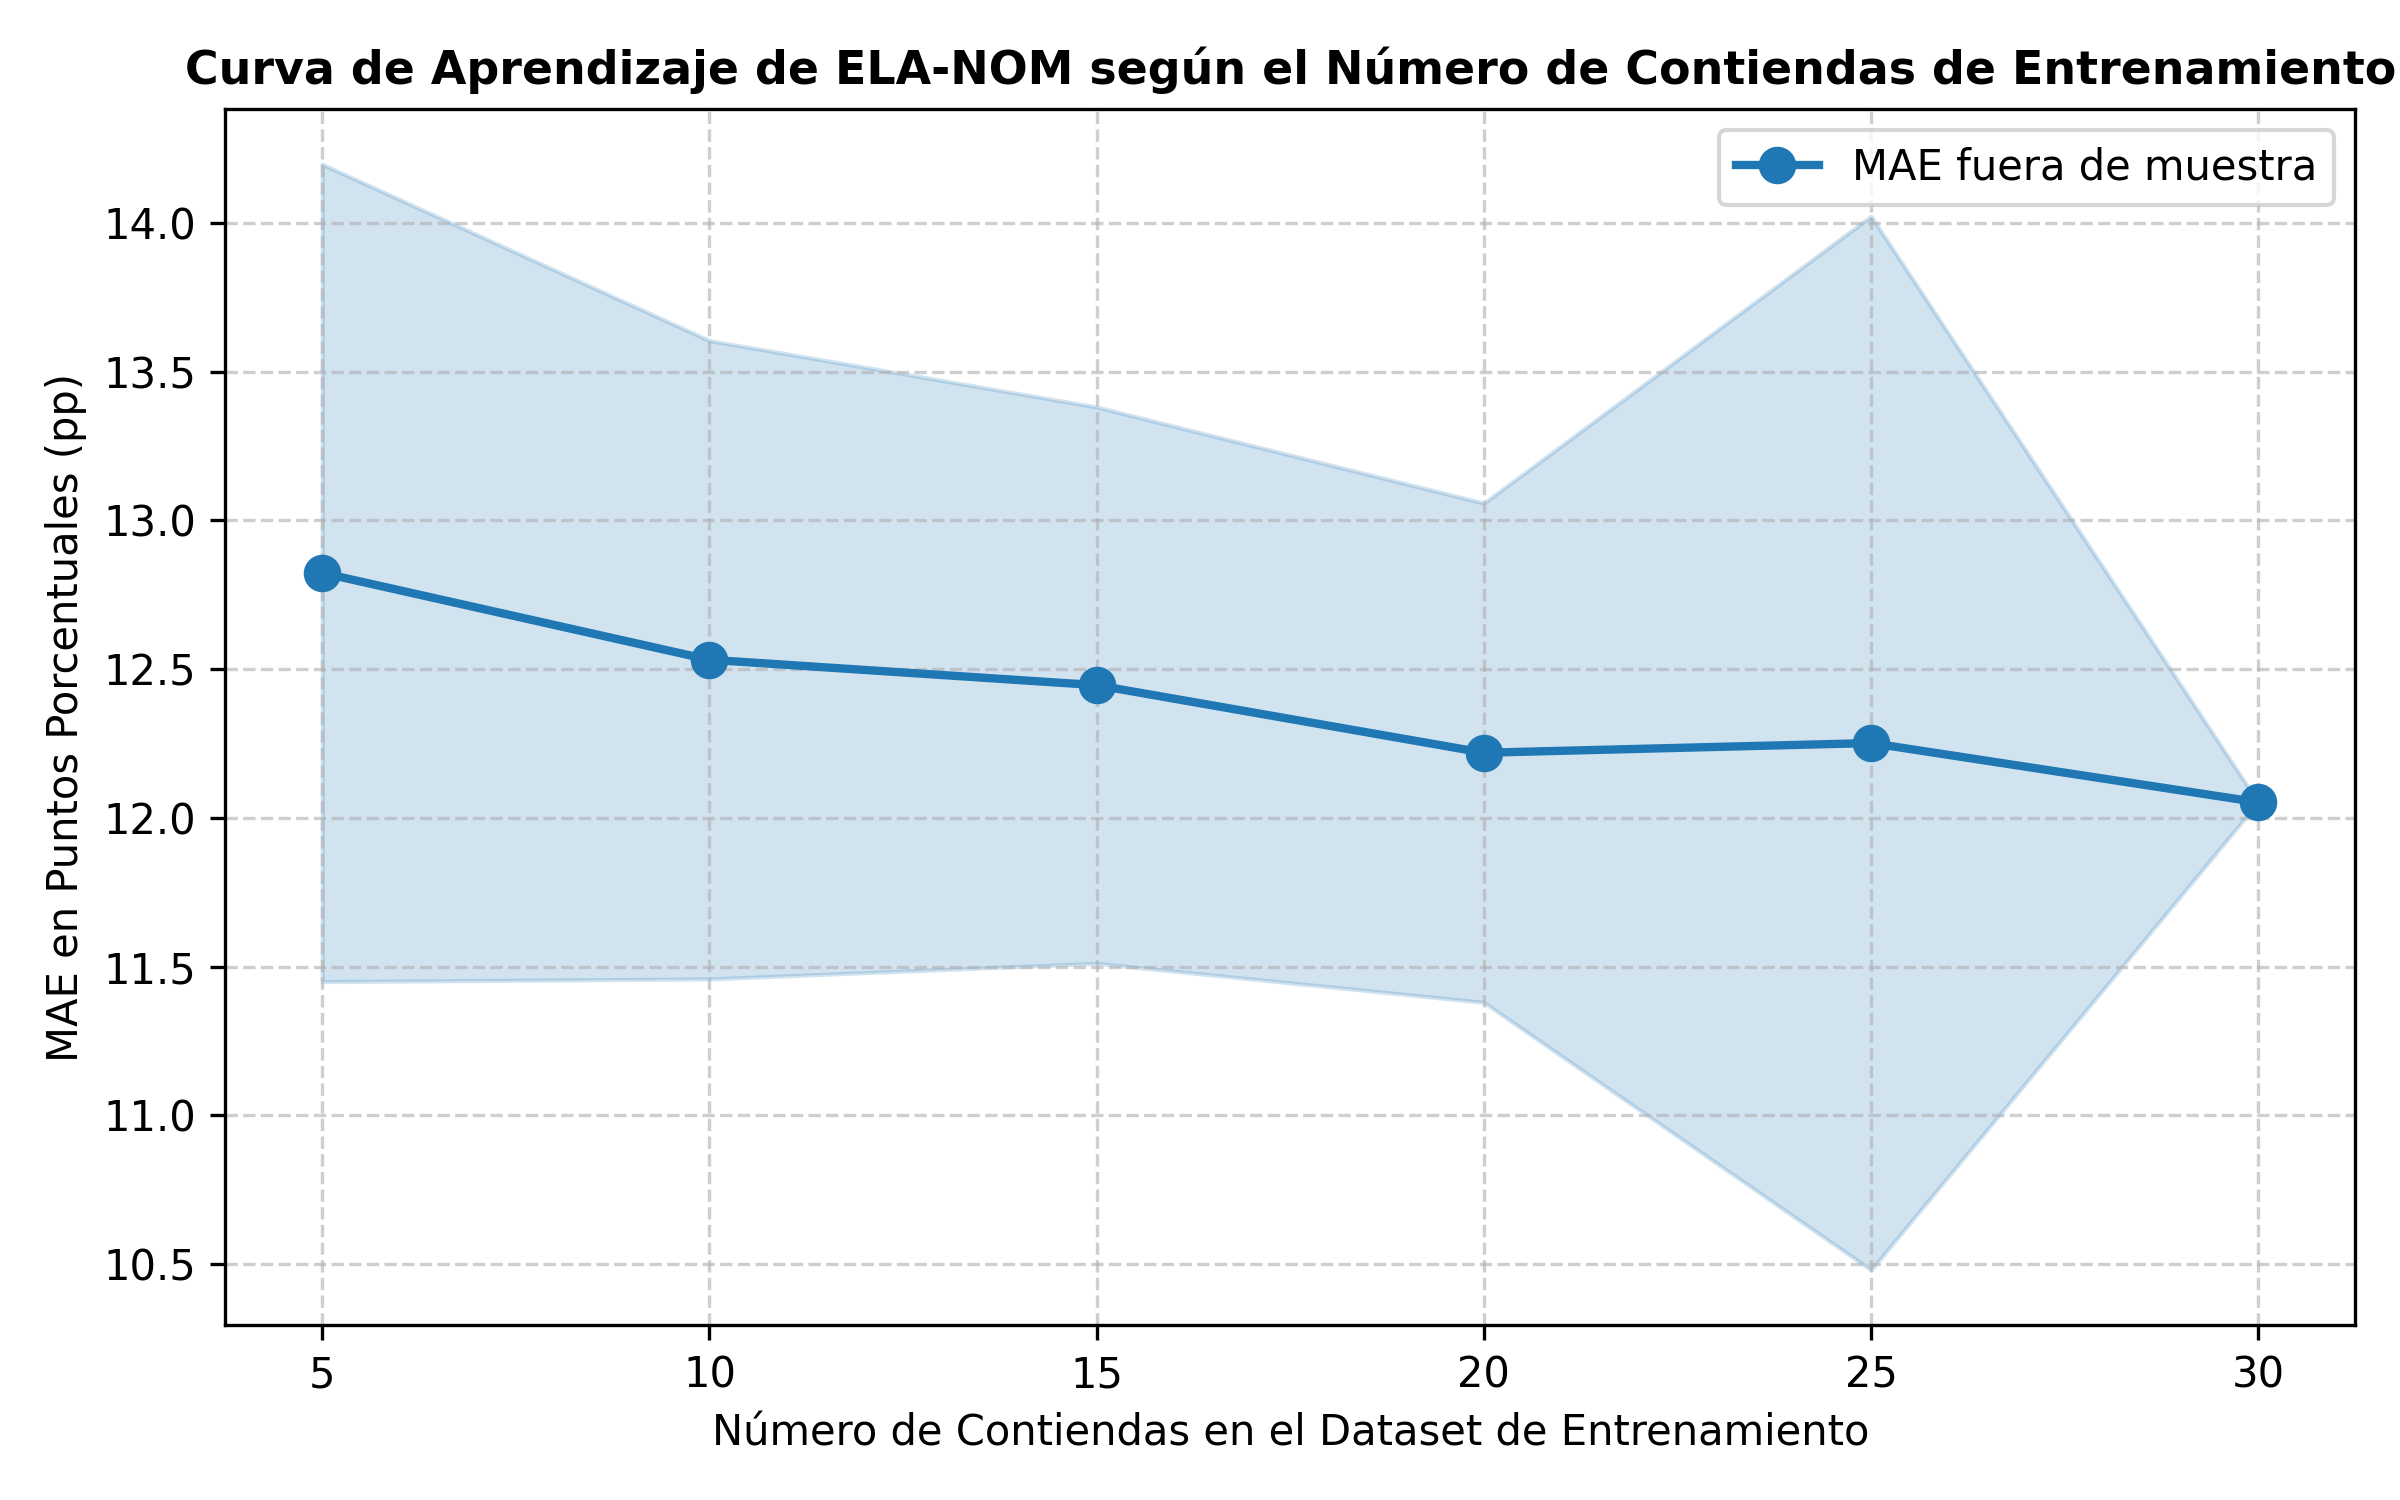
\includegraphics[width=0.82\linewidth]{img/col_learning_curve.png}
\caption{Curva de aprendizaje de ELA-NOM. MAE fuera de muestra (media y banda $\pm 1$ desviación estándar) en función del número de contiendas de entrenamiento. La banda sombreada representa la variabilidad entre las 50 repeticiones de muestreo.}
\label{fig:col_learning_curve}
\end{figure}

La reducción total del MAE entre el escenario de menor muestra (5~contiendas) y la muestra completa (30~contiendas) es de apenas \textbf{0{,}77~pp} (de 12{,}82 a 12{,}05~pp). La curva es prácticamente plana: con tan solo 10~contiendas se alcanza un MAE de 12{,}53~pp, y los incrementos marginales siguientes son de décimas de punto porcentual. Adicionalmente, a $N=25$ la desviación estándar sube a 1{,}77~pp, lo que indica inestabilidad en algunos subconjuntos específicos de esa talla, probablemente derivada del pequeño universo de 30~municipios disponibles.

La interpretación más honesta de este resultado es que el piso de error del modelo (~12~pp) no está determinado por la insuficiencia de datos de entrenamiento, sino por el nivel de ruido intrínseco de la señal digital como predictor de cuota de voto. Esto tiene una consecuencia metodológica positiva: el modelo no requiere grandes acervos históricos para funcionar, siendo viable desde tamaños de muestra moderados; y una consecuencia negativa: agregar más elecciones del mismo tipo no resolverá el error residual observado.

\subsubsection*{P3 (complementario): \textquestiondown{}La tracción tardía aporta información predictiva adicional sobre la dominancia relativa?}

Se comparó la correlación de Spearman entre la cuota de voto real y dos versiones de la señal digital: (i)~la dominancia acumulada durante la ventana completa de 14~días antes de la elección, y (ii)~la dominancia de crecimiento tardío (últimos días de campaña, reportada como \textit{late\_growth} en las plataformas disponibles).

Los resultados fueron:
\begin{itemize}
    \item Dominancia acumulada 14~días: $\rho = 0{,}7036$
    \item Dominancia de tracción tardía: $\rho = 0{,}6655$
\end{itemize}

La diferencia entre ambos coeficientes es de $\Delta\rho = 0{,}038$. Con $n=109$ candidatos no se realizó un test de Steiger formal, pero la magnitud de la diferencia es pequeña en términos prácticos. Esta evidencia sugiere que la tracción tardía \textbf{no aporta información predictiva adicional} sobre la señal acumulada: la dominancia relativa de \textit{likes} en la ventana de 14~días ya captura la mayor parte de la señal disponible. La decisión de diseño de ELA-NOM de trabajar con la ventana acumulada en lugar de ponderar de forma diferencial los días finales queda así respaldada empíricamente, aunque los datos disponibles no permiten una verificación estadística concluyente dada la escala de la muestra.

% ──────────────────────────────────────────────────────────────
\section{Síntesis: contribuciones al estado del arte}
% ──────────────────────────────────────────────────────────────

Los hallazgos empíricos y los desarrollos técnicos documentados a lo largo de este estudio confluyen en cuatro contribuciones sustanciales al dominio de la analítica política y los modelos predictivos heterodoxos:

\begin{enumerate}
    \item \textbf{Elección-Agnosticismo Empírico:} Se establece una ruta metodológica viable, demostrada a través de la regresión fraccional basada en la métrica transversal de dominancia relativa, para superar la limitación de no transferibilidad del SOMEN-DC (tercera limitación identificada en la Sección~1.2), permitiendo entrenar algoritmos con observaciones de múltiples contiendas de alcaldías simultáneas y abstraer reglas de decisión exportables a elecciones de distinto formato.
    
    \item \textbf{Total Independencia Demoscópica:} A diferencia de la inmensa mayoría de la literatura contemporánea en estimación digital electoral, este esquema sustituye la obligatoriedad de usar encuestas como variable dependiente, anclando directamente su optimización sobre la variable \textit{ground truth} universal: el escrutinio final. 
    
    \item \textbf{Restaurador Temporal de Series (Modelo Weibull):} Se introduce y formaliza una arquitectura matemática de interpolación capaz de retrotraer variables acumulativas hacia instantes en el pasado. Esto resuelve el que quizás sea el mayor obstáculo técnico para la investigación retrospectiva de dinámicas digitales, facultando a los analistas a poblar \textit{datasets} de series temporales históricas partiendo exclusivamente de una extracción actual estática, sin requerir despliegues preventivos costosos. La solución está calibrada sobre el panel de Costa Rica 2026 y su generalización a otras elecciones debe verificarse empíricamente.
    
    \item \textbf{Democratización del \textit{Pipeline}:} Se verifica la operatividad de la solución utilizando, de principio a fin, una orquestación ligera ensamblada con herramientas de mercado genéricas (\textit{Make}, \textit{Apify}, API oficiales, librerías \textit{Headless}), mostrando que la predicción y monitoreo algorítmico no requiere necesariamente infraestructuras corporativas, gubernamentales o institucionales avanzadas.
\end{enumerate}
